\documentclass{article}
\usepackage{amsmath,amssymb,tikz}
\usetikzlibrary{arrows.meta,tikzmark}
\begin{document}

\begin{align*}
x\tikzmark{x}(t)*h\tikzmark{h}(t) &= y\tikzmark{y}(t) \\[2em]
X(f) \, H(f) &= Y(f) 
\end{align*}

\begin{tikzpicture}[overlay,remember picture, > = {Circle[open,blue]}]
  \draw [<->] ([yshift=-.7ex]pic cs:x) -- ++(0,-2.2em);
  \draw [<->] ([yshift=-.7ex]pic cs:h) -- ++(0,-2.2em);
  \draw [<->] ([yshift=-.7ex]pic cs:y) -- ++(0,-2.2em);
\end{tikzpicture}

\end{document}